\newpage
\section{Proofs}
\label{app:theory_proofs}

\subsection{Proof of Theorem~\ref{thm:return_decomposition}}
\label{app:proof_return_improvement}

\begin{proof}
Define the student's finite-horizon value and advantage functions by
\begin{align*}
V_t^{\pi_S}(h)
&:=\mathbb E_{a\sim\pi_S(\cdot\mid h)}Q_t^{\pi_S}(h,a),\\
A_t^{\pi_S}(h,a)
&:=Q_t^{\pi_S}(h,a)-V_t^{\pi_S}(h),
\end{align*}
with $V_H^{\pi_S}=0$.

\paragraph{Step 1: derive the finite-horizon performance-difference identity.}
By the Bellman definition of $Q_t^{\pi_S}$,
\[
Q_t^{\pi_S}(h_t,a_t)
=\mathbb E\!\left[r_t+V_{t+1}^{\pi_S}(h_{t+1})
\mid h_t,a_t\right].
\]
Taking expectation under the assisted trajectory and summing over turns gives
\begin{align*}
\sum_{t=0}^{H-1}\mathbb E_{\pi_G}\!\left[A_t^{\pi_S}(h_t,a_t)\right]
&=\sum_{t=0}^{H-1}\mathbb E_{\pi_G}\!\left[
r_t+V_{t+1}^{\pi_S}(h_{t+1})-V_t^{\pi_S}(h_t)\right]\\
&=J(\pi_G)-J(\pi_S).
\end{align*}
The value terms telescope because the policies share the distribution of initial task inputs and $V_H^{\pi_S}=0$.

\paragraph{Step 2: evaluate the advantage at an intervention turn.}
Condition on $(t,h_t)$ and sample the student proposal and teacher action as in the proposal-coupled construction. Since $a_t=a_t^S$ when $I_t=0$ and $a_t=a_t^T$ when $I_t=1$,
\begin{align*}
&\mathbb E\!\left[A_t^{\pi_S}(h_t,a_t)\mid h_t\right]\\
&=\mathbb E\!\left[
I_tA_t^{\pi_S}(h_t,a_t^T)+(1-I_t)A_t^{\pi_S}(h_t,a_t^S)
\,\middle|\,h_t\right]\\
&=\mathbb E\!\left[
I_t\bigl(A_t^{\pi_S}(h_t,a_t^T)-A_t^{\pi_S}(h_t,a_t^S)\bigr)
\,\middle|\,h_t\right]\\
&=\mathbb E\!\left[
I_t\bigl(Q_t^{\pi_S}(h_t,a_t^T)-Q_t^{\pi_S}(h_t,a_t^S)\bigr)
\,\middle|\,h_t\right].
\end{align*}
The third line uses $\mathbb E[A_t^{\pi_S}(h_t,a_t^S)\mid h_t]=0$; the final line cancels the common value term.

\paragraph{Step 3: aggregate over the assisted trajectory.}
Substituting Step 2 into Step 1 and applying the law of total expectation gives Eq.~\ref{eq:return_decomposition}.

Under Assumption~\ref{ass:average_recoverability}, multiplying
Eq.~\ref{eq:average_recoverability} by
$\mathbb E_{\pi_G}[N_{\mathrm{int}}]$ and applying the theorem yields
\[
J(\pi_G)-J(\pi_S)
\ge\gamma\,\mathbb E_{\pi_G}[N_{\mathrm{int}}]\ge0,
\]
which proves the lower bound in Theorem~\ref{thm:return_decomposition}. If the expected number of
interventions is zero, $\pi_G=\pi_S$ almost surely and the same conclusion
holds directly.
\end{proof}

\subsection{Proof of Proposition~\ref{prop:corrective_supervision}}
\label{app:proof_corrective_supervision}

\begin{proof}
Fix a history $h$ at a terminal decision turn $t$. There are three actions $\{a,b,c\}$ with rewards $r(a)=r(b)=1$ and $r(c)=0$, so $Q_t^{\pi_S}(h,i)=r(i)$. Suppress $h$ in the distributions and use the unrestricted softmax parameterization
\[
p_i(\theta)=\frac{\exp(\theta_i)}{\sum_{j\in\{a,b,c\}}\exp(\theta_j)}.
\]
Initialize $\theta_0=(0,0,0)$, so $p=\pi_S=(1/3,1/3,1/3)$. The three logits are independent parameters. Choose a teacher
\[
u=\pi_T=\bigl(v(1-\epsilon),v\epsilon,1-v\bigr),
\qquad
\frac23<v<1,\quad 0<\epsilon<\frac12,
\]
with
\begin{equation}
v^2\epsilon(1-\epsilon)<(1-v)^2.
\label{eq:corrective_teacher_family}
\end{equation}
For any $v\in(2/3,1)$, this condition holds for sufficiently small positive $\epsilon$. Thus the construction describes a family of full-support teachers, each with return $v>2/3=J_{t,h}(\pi_S)$. Every teacher in this family is represented by the student class, for example by logits $\theta_i=\log u_i$.

Write $\ell_i=\log(p_i/u_i)$ and $\bar\ell=\sum_i p_i\ell_i$. The ordinary logit gradients of the two losses in Proposition~\ref{prop:corrective_supervision} are
\begin{equation}
G_{\mathrm{OPD},i}=p_i(\ell_i-\bar\ell),
\qquad
G_{\mathrm{SFT},i}=p_i-u_i.
\label{eq:corrective_gradients}
\end{equation}
Both gradients sum to zero. The first follows by differentiating $\sum_i p_i\log(p_i/u_i)$ and using $\nabla_\theta\log p_i=e_i-p$; the second is the expected teacher-action SFT gradient. For $M\in\{\mathrm{OPD},\mathrm{SFT}\}$, the updated logits are $\theta_M^+=\theta_0-\alpha G_M$, and $\pi_M^+=\operatorname{softmax}(\theta_M^+)$.

The softmax Jacobian is $F=\operatorname{diag}(p)-pp^\top$. At the uniform initial policy, $F=\frac13 I-\frac19\mathbf1\mathbf1^\top$, hence the first-order probability change under update $M$ is
\[
\left.\frac{d}{d\alpha}\pi_M^+\right|_{\alpha=0}
=-FG_M=-\frac13G_M.
\]
Since the reward vector is $(1,1,0)$ and $\sum_iG_{M,i}=0$, the return derivative equals $G_{M,c}/3$. Therefore
\begin{align}
\left.\frac{d}{d\alpha}J_{t,h}(\pi_{\mathrm{OPD}}^+)\right|_{\alpha=0}
&=\frac1{27}\log\frac{u_a u_b}{u_c^2}
=\frac1{27}\log\frac{v^2\epsilon(1-\epsilon)}{(1-v)^2}<0,\notag\\
\left.\frac{d}{d\alpha}J_{t,h}(\pi_{\mathrm{SFT}}^+)\right|_{\alpha=0}
&=\frac{v-2/3}{3}>0.
\label{eq:corrective_return_derivatives}
\end{align}

Let $d_{\mathrm{OPD}}$ be the negative of the first derivative and $d_{\mathrm{SFT}}$ the second derivative in Eq.~\ref{eq:corrective_return_derivatives}. Both are strictly positive. Smoothness gives
\begin{align*}
J_{t,h}(\pi_{\mathrm{OPD}}^+)
&=J_{t,h}(\pi_S)-d_{\mathrm{OPD}}\alpha+O(\alpha^2),\\
J_{t,h}(\pi_{\mathrm{SFT}}^+)
&=J_{t,h}(\pi_S)+d_{\mathrm{SFT}}\alpha+O(\alpha^2).
\end{align*}
Choose $\alpha_0>0$ small enough that each remainder has magnitude at most $d_M\alpha/2$ for every $0<\alpha\le\alpha_0$. The OPD update then strictly decreases return, while the SFT update strictly increases it, proving Eq.~\ref{eq:corrective_supervision_separation}.

All probabilities are positive, and the teacher advantage and derivative inequalities are strict. By continuity, these inequalities persist under sufficiently small perturbations of the initial logits and teacher probabilities. The comparison concerns the update direction: both population losses admit the representable teacher as a global minimizer.
\end{proof}

\section{Mode Seeking and Mode Covering}
\label{app:mode_balance}

Figure~\ref{fig:mode_balance} illustrates the different optimization tendencies of the two KL directions at a fixed interaction history. Reverse KL emphasizes actions already sampled by the student and favors concentrating probability on teacher-supported modes. Forward KL penalizes low student probability on actions supported by the teacher, encouraging coverage of behaviors the student rarely generates. UOPD applies reverse KL to retained student actions and implements forward KL through SFT on teacher corrections. Executing these corrections also changes subsequent interaction histories; this effect on the rollout comes from action replacement, while SFT provides the learning signal.

\begin{figure}[htbp]
\centering
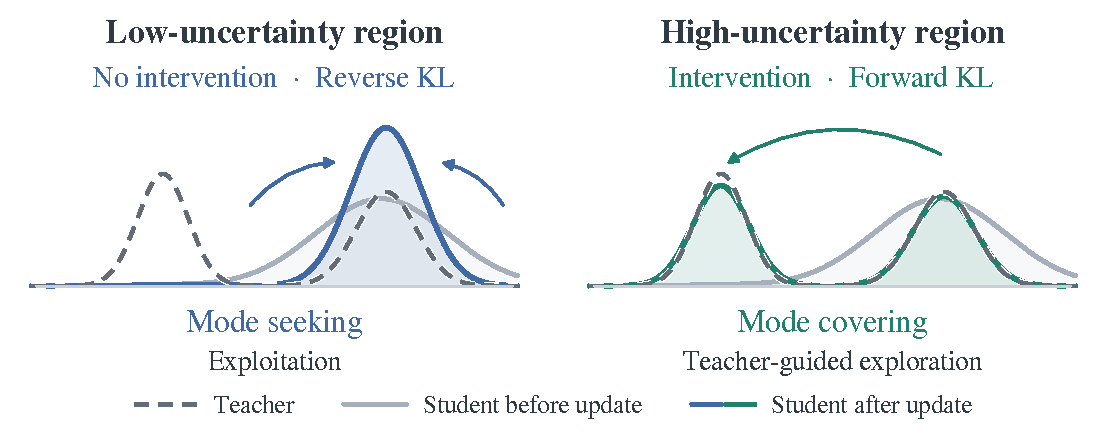
\includegraphics[width=\linewidth]{figures/uai_opd_mode_balance.pdf}
\caption{\textbf{Mode seeking and mode covering in UOPD.}
Left: reverse KL refines student probability around a teacher-supported mode.
Right: forward KL encourages the student to cover teacher behaviors it rarely generates.
The curves schematically illustrate the two loss directions rather than measured policy distributions.}
\label{fig:mode_balance}
\end{figure}
\FloatBarrier

\section{Details of the ALFWorld Motivation Study}
\label{app:motivation_details}

This section provides the protocol for the controlled study in
Section~\ref{sec:motivation}. We compare student-only rollouts, one teacher
intervention at a low-confidence step, and one teacher intervention at a random
step. Both models remain fixed, so the comparison measures how an action
correction changes subsequent student behavior without a parameter update.

\subsection{Models, Tasks, and Rollout Collection}

We collect student-only rollouts on 100 tasks from the ALFWorld valid-seen split
\citep{shridhar2021alfworld}. The student is Qwen2.5-3B-Instruct, evaluated
zero-shot, and the teacher is GiGPO-Qwen2.5-7B-Instruct-ALFWorld
\citep{feng2025gigpo}. Episodes terminate on task completion or after 50
environment turns. We use sampling temperature $0.4$, a maximum of 512 response
tokens per turn, and seed 42. Each response contains reasoning and an environment
action; the resulting observation is appended to the interaction history.
We save the exact prompt and response token IDs and score the recorded student
responses under the teacher after rollout collection.

\subsection{Teacher Confidence and Intervention Selection}

For a student response $a_t^S=(y_{t,1},\ldots,y_{t,L_t})$ at turn $t$, we define
teacher confidence as the length-normalized log-probability
\begin{equation}
C_t := \frac{1}{L_t}\sum_{j=1}^{L_t}
\log\pi_T(y_{t,j}\mid h_t,y_{t,<j}),
\label{eq:app_teacher_confidence}
\end{equation}
where $h_t$ is the interaction history defined in Section~\ref{subsec:preliminary}. We score all response
tokens, including reasoning and the structured action, and exclude prompt
tokens. Scores are computed from unscaled teacher logits and reported in nats
per token; higher values indicate greater teacher support for the student
response. The corresponding uncertainty score is $\delta_t=-C_t$.

We set $\tau_C$ to the 25th percentile of valid turn-level confidence scores
across the 100 baseline rollouts, giving $\tau_C\approx-1.216$. For trajectory
$i$ with $H_i$ recorded turns, the selected intervention turn is
\begin{equation}
t_i^* := \min\{t:1\le t<H_i-1,\ C_{i,t}<\tau_C\}.
\label{eq:app_motivation_trigger}
\end{equation}
Turn indices are zero-based. This selects the first eligible threshold crossing,
rather than the single lowest-confidence action. We exclude the first and final
baseline turns to retain a replay prefix and subsequent student actions for
comparison. Of the 100 baseline trajectories, 96 meet this criterion and 93 have
verified matching intervention replays. We use these same 93 tasks for all
three comparison conditions.

\subsection{Matched Single-Turn Interventions}

The \textbf{Student} condition uses the original student-only trajectory.
The \textbf{Intervention} condition replaces the action at $t_i^*$ with one
teacher-generated action. The \textbf{Random} condition instead samples one
turn uniformly from $\{1,\ldots,H_i-2\}$ on the same baseline trajectory,
using a task-specific random seed derived from seed 42.

For either intervention condition, we reset the environment to the recorded game
file and execute the saved student actions up to the chosen turn. The teacher
then generates and executes one action, and the student resumes until task
completion or the original 50-turn limit. The intervened rollout therefore
shares the baseline prefix and receives exactly one turn of teacher assistance.
We match trajectories by game file and reconstructed model inputs, and verify
replays against the saved prompts, actions, and final rewards. When Random and
Intervention choose the same turn, they share the saved teacher branch; this
occurs on four tasks, leaving 275 distinct trajectories across the three
conditions.

\subsection{Measurements in Figure~\ref{fig:motivation}}

\paragraph{Teacher confidence.}
Panel (a) averages $C_t$ over baseline trajectories that reach each displayed
turn, using the full set of 100 student-only rollouts. Panel (b) aligns the
matched Student and Intervention trajectories at $t_i^*$ and averages teacher
confidence on student-generated responses at offsets $1,\ldots,5$. The teacher's
replacement action is excluded from this readout. Each mean uses the trajectories
with an available response at that turn; trajectories that have already ended
are not padded. We plot turns with at least 15 observations and connect the
means without smoothing.

\paragraph{Task success.}
Panel (c) reports the percentage of the 93 matched tasks completed successfully
under each condition, using the environment's terminal success indicator.

\paragraph{State returns.}
Panel (d) reports the percentage of trajectories that leave a state and later
return to it. Let $z_0,\ldots,z_H$ denote the symbolic states before the first
action and after each executed action. We identify a state by its exact set of
raw PDDL facts, including predicate names, argument identities and types, and
simulator bookkeeping facts. Observation text, turn numbers, and interaction
history are excluded from this identity. For each trajectory, we compute
\[
I_{\mathrm{return}}(\tau)
=\mathbf{1}\!\left\{\exists\,t\in\{1,\ldots,H\}:
 z_t\ne z_{t-1}\ \text{and}\ z_t\in\{z_0,\ldots,z_{t-1}\}\right\}.
\]
This statistic is computed within each trajectory and covers the full rollout,
including the teacher action where present. Consecutive unchanged states do not
count as a return, and returning does not require repeating the same action.
State returns provide a task-specific indicator of backtracking; a return can
also accompany useful information gathering.
Table~\ref{tab:motivation_protocol} summarizes task success and state returns for all three conditions.

\begin{table}[ht]
\centering
\small
\begin{tabular}{lrr}
\toprule
Condition & Task success (\%) & Trajectories with state returns (\%) \\
\midrule
Student      & 13.98 ($13/93$) & 93.55 ($87/93$) \\
Random       & 16.13 ($15/93$) & 91.40 ($85/93$) \\
Intervention & 25.81 ($24/93$) & 80.65 ($75/93$) \\
\bottomrule
\end{tabular}
\caption{Outcomes on the same 93 ALFWorld tasks used in
Fig.~\ref{fig:motivation}(c,d). Random and Intervention each execute one teacher
action before returning control to the student.}
\label{tab:motivation_protocol}
\end{table}

\section{Experimental Details}
\label{app:provenance}

This section describes the benchmarks and data, the student and teacher models, the baselines, and
the training and evaluation configurations behind the results in Section~\ref{sec:experiments}.
Appendix~\ref{app:prompts} gives the prompts used for training and evaluation.

\subsection{Benchmark Environments}
\label{app:data}

\paragraph{ALFWorld} \citep{shridhar2021alfworld}. Text-based household tasks of six types (pick,
clean, heat, cool, examine, pick-two) in the TextWorld engine. Training draws from the $3{,}553$
training games. We evaluate on the $140$ seen and $134$ unseen validation tasks. A task succeeds when
it is completed within $50$ environment steps, and an episode's turns are its environment steps, with
a failed episode counting the full $50$.

\paragraph{WebShop} \citep{yao2022webshop}. Instruction-following product search and purchase over the
$1{,}000$-product catalog. Training draws from a pool of $6{,}410$ instructions, and evaluation uses
$128$ test instructions that are disjoint from the pool and shared by every method. The task score is
the environment's attribute-match reward on a $0$--$100$ scale, the success rate is the share of
episodes with a perfect match, and the episode cap is $15$ steps.

\paragraph{Search} \citep{jin2025searchr1}. Open-domain question answering with a retrieval tool, in
the Search-R1 setting. Training draws from $169{,}615$ questions ($79{,}168$ from NQ and $90{,}447$
from HotpotQA). The test set is Search-R1's four multi-hop datasets, $22{,}523$ questions in total:
HotpotQA ($7{,}405$), 2WikiMultiHopQA ($12{,}576$), MuSiQue ($2{,}417$) and Bamboogle ($125$). Retrieval uses Search-R1's e5-base-v2 encoder over its 2018 Wikipedia
corpus with a flat FAISS index, returning the top $3$ passages per query. Answers are scored by exact
match after normalisation against any gold answer, using the last \texttt{<answer>} of the episode.
The turn limit is $8$.

\subsection{Students and Teachers}
\label{app:models}

\begin{center}\small
\begin{tabular}{@{}l l l@{}}
\toprule
Benchmark & Students & Teacher \\
\midrule
ALFWorld & Qwen2.5-3B-Instruct, Qwen2.5-1.5B-Instruct & GiGPO-Qwen2.5-7B-Instruct-ALFWorld \\
WebShop & Qwen2.5-3B-Instruct, Qwen2.5-1.5B-Instruct & GiGPO-Qwen2.5-7B-Instruct-WebShop \\
Search & Qwen2.5-1.5B (base) & SearchR1-qwen2.5-7b-em-ppo \\
\bottomrule
\end{tabular}
\end{center}

\noindent The ALFWorld and WebShop teachers are RL-trained with GiGPO \citep{feng2025gigpo}; the Search
teacher is Search-R1's PPO-trained $7$B model, trained from a base checkpoint on Search-R1's raw
prompt, so the Search student is a base checkpoint prompted the same way. In every pair, teacher and
student share a tokenizer, so the teacher can score the student's own tokens.

\subsection{Baselines}
\label{app:baselines}

\paragraph{Zero-shot student and teacher.} Evaluated without training under the protocol of
Appendix~\ref{app:evaluation-protocol}. They bound the results from below and above.

\paragraph{OPD} \citep{agarwal2024policy,lu2025onpolicydistillation}. The student plays the whole
episode, and the teacher scores every student token under the same prompt. Each token receives the
advantage $A_t = \lambda\,(\log\pi_T(y_t) - \log\pi_{S,\mathrm{old}}(y_t))$ with $\lambda=1$, optimised
with a PPO objective (clip $0.2$, dual clip $3.0$, token-mean aggregation). UOPD uses the same
distillation term and adds its intervention rule and the SFT loss on intervened turns.

\paragraph{TCOD-F2B and TCOD-B2F} \citep{wang2026exploring}. Temporal curricula over the rollout horizon,
advanced every $\eta$ rollout batches $n$. F2B lets the student play only the first
$W_n = \min(1+\lfloor n/\eta\rfloor,\,T_{\max})$ turns of an episode and then ends it. B2F replays a
stored expert prefix of $P_n = \mathrm{clamp}(L-1-\lfloor n/\eta\rfloor,\,0,\,L-1)$ actions, where $L$ is
the expert trajectory's length, and the student plays from that point on. The prefix carries no loss.
Both train the student's turns with the OPD loss and are evaluated on the full horizon. On ALFWorld,
$\eta$ is $6$ for F2B and $5$ for B2F.

\paragraph{FTB-OPD} \citep{futurebridgeopd2026}. Introduces teacher corrections at steps where the
student and teacher disagree most, and keeps a correction for distillation only when it improves the
teacher's preference over the student's subsequent continuations. Validating a correction requires
paired student continuations, which is the source of its extra training time in
Figure~\ref{fig:training-time-3b}.

\subsection{Training Configuration}
\label{app:training-config}

We implement UOPD using Trinity-RFT \citep{pan2025trinityrft}.
We use its asynchronous rollout and training
pipeline, with vLLM for student and teacher inference and the verl backend
with fully sharded data parallelism (FSDP) for student
updates. Table~\ref{tab:app-gpu-allocation} gives the eight-GPU allocation.

For ALFWorld and WebShop, the primary UOPD schedules linearly reduce the target intervention
rate from $30\%$ to $5\%$ for the $3$B student and from $50\%$ to $30\%$ for the $1.5$B student.
The intervention threshold is calibrated online using teacher confidence on student-proposed actions.
The SFT weight, teacher execution, and intervention schedules are compared in
Section~\ref{subsec:exp-ablation}. Table~\ref{tab:app-train-hparams} lists the full configuration.

\paragraph{Intervention signals.}
For a student-proposed action $a_t^S$ at history $h_t$, the teacher-confidence
signal is the teacher's length-normalized negative log-likelihood:
\[
\delta_t^{\mathrm{conf}}
=-\frac{\log\pi_T(a_t^S\mid h_t)}{|a_t^S|}.
\]
The student--teacher confidence gap is
\[
\delta_t^{\mathrm{gap}}
=\frac{\log\pi_\theta(a_t^S\mid h_t)-\log\pi_T(a_t^S\mid h_t)}{|a_t^S|}.
\]
Here $|a_t^S|$ is the number of tokens in the action response, and
$\pi_\theta$ is the student policy used to generate the action.
Larger scores indicate lower teacher confidence or a larger student--teacher
confidence gap, respectively; both trigger intervention when they exceed
$\tau_n$.

\begin{table}[!ht]
\centering
\caption{\textbf{Training hyperparameters.} Settings shared by all methods are listed first; the
last block is specific to UOPD.}
\label{tab:app-train-hparams}
\scriptsize
\setlength{\tabcolsep}{4pt}
\begin{tabular}{@{}l c c c@{}}
\toprule
 & ALFWorld & WebShop & Search \\
\midrule
\multicolumn{4}{@{}l}{\emph{Optimisation}} \\
Optimizer & \multicolumn{3}{c}{AdamW, $\beta{=}(0.9, 0.999)$, weight decay $0.01$, constant learning rate, no warm-up} \\
Learning rate & $1\times10^{-6}$ & $1\times10^{-6}$ & $1\times10^{-6}$ \\
Gradient clipping & $1.0$ & $1.0$ & $1.0$ \\
Training steps & $250$ & $150$ & $300$ \\
Tasks per rollout batch & $16$ & $16$ & $64$ \\
Rollouts per task & $1$ & $1$ & $1$ \\
Update epochs / mini-batch & $1$ / $64$ & $1$ / $64$ & $1$ / $64$ \\
Dynamic batching (tokens per GPU) & $16{,}384$ & $16{,}384$ & $9{,}728$ \\
Sampling & \multicolumn{3}{c}{asynchronous, at most $2$ policy versions stale} \\
\midrule
\multicolumn{4}{@{}l}{\emph{Loss}} \\
Distillation (reverse-KL) coefficient $\lambda$ & $1.0$ & $1.0$ & $1.0$  \\
\midrule
\multicolumn{4}{@{}l}{\emph{Rollout}} \\
Max prompt / response tokens & $2{,}048$ / $512$ & $4{,}096$ / $512$ & $4{,}096$ / $512$\\
Sampling temperature & $1.0$ & $1.0$ & $1.0$ \\
Episode limit (steps / turns) & $50$ & $15$ & $8$ \\
History in the prompt & last $2$ steps & last $2$ steps & full episode \\
Retrieval & -- & -- & top $3$ passages \\
\midrule
\multicolumn{4}{@{}l}{\emph{UOPD}} \\
Intervention signal & Teacher confidence & Teacher confidence & Confidence gap \\
Scoring temperature for the signal & $1.0$ & $1.0$ & $1.0$ \\
Intervention schedule, $3$B & $30\%\!\to\!5\%$ over $120$ & $30\%\!\to\!5\%$ over $75$ & -- \\
Intervention schedule, $1.5$B & $50\%\!\to\!30\%$ over $120$ & $50\%\!\to\!30\%$ over $75$ & constant $30\%$ \\
SFT weight $\beta$, form & $1.0$ & $1.0$ & $1.0$\\
\bottomrule
\end{tabular}
\\[3pt]
\end{table}

\begin{table}[!ht]
\centering
\caption{\textbf{Eight-GPU allocation.}
Student rollout, teacher inference, and student updates run on separate GPU groups.}
\label{tab:app-gpu-allocation}
\small
\setlength{\tabcolsep}{5pt}
\begin{tabular}{@{}l c l@{}}
\toprule
Role & GPUs & Configuration \\
\midrule
Student rollout (vLLM) & $4$ & $2$ engines, tensor parallel size $2$ per engine \\
Teacher inference (vLLM) & $2$ & $1$ engine, tensor parallel size $2$ \\
Student updates (verl/FSDP) & $2$ & Ulysses sequence parallel size $2$ \\
\midrule
Total & $8$ & Single node \\
\bottomrule
\end{tabular}
\end{table}

\subsection{Evaluation Protocol}
\label{app:evaluation-protocol}

\paragraph{ALFWorld.} We evaluate household task completion on $140$ seen and $134$ unseen
tasks, reporting the percentage of successfully completed tasks in each split. Average turns
are computed separately for each split over all episodes, including failures.

\paragraph{WebShop.} We use the $1000$-product catalog and $128$ test tasks. Task score measures
how well the selected product satisfies the request; success rate measures full task completion.
Average turns include both successful and failed episodes.
For ALFWorld and WebShop, Table~\ref{tab:exp-agentic} reports means and standard deviations
over three evaluation seeds.

\paragraph{Search.} Figure~\ref{fig:search-15b-multihop} reports exact match on each of the four
multi-hop test sets of Search-R1 \citep{jin2025searchr1}: HotpotQA, 2WikiMultiHopQA, MuSiQue and
Bamboogle, $22{,}523$ questions in total. Average turns are computed over the same $22{,}523$
questions. A turn is one model response, the answering one included, so an episode that reaches the
limit and receives the forced answer counts nine turns.
Both OPD and UOPD use seed $42$, greedy decoding, forced answers, and an eight-turn limit.

\begin{center}\small
\begin{tabular}{@{}l c c c@{}}
\toprule
 & ALFWorld & WebShop & Search \\
\midrule
Temperature & $0.4$ & $0.4$ & $0$ (greedy) \\
Max prompt / response tokens & $2{,}048$ / $512$ & $4{,}096$ / $512$ & as in training / $512$ \\
Episode limit & $50$ & $15$ & $8$, then a forced answer \\
Test set & $140$ seen, $134$ unseen & $128$ test & $22{,}523$ multi-hop questions \\
\bottomrule
\end{tabular}
\end{center}

\noindent Every evaluation uses the checkpoint of the final training step. A Search episode that
reaches the turn limit without an answer is given one additional turn that asks for the final answer
(Appendix~\ref{app:prompt-search}); this turn is used only at evaluation.


\subsection{Hardware}

Training runs use a single node, primarily with eight NVIDIA RTX PRO 6000
Blackwell GPUs. We also use four-GPU setups with NVIDIA H100 (80\,GB) or
NVIDIA RTX A6000 (48\,GB) GPUs. All reported training-time comparisons use the
eight-GPU RTX PRO 6000 Blackwell setup, with the allocation in
Table~\ref{tab:app-gpu-allocation}.

\section{Environment Prompts}
\label{app:prompts}

This section gives the prompts used for each environment during training and evaluation, verbatim.
Braces mark the fields filled at each step. The student and the teacher receive the identical prompt,
which lets the teacher score the student's own tokens, and each prompt is sent as a single
chat-formatted user message. We pass no system message, so the model's chat template adds its default
one: ``You are Qwen, created by Alibaba Cloud. You are a helpful assistant.'' for the Qwen2.5-Instruct
students, and ``You are a helpful assistant.'' for the base Search student. No prompt states the step
or turn limit; the environment enforces it.

\subsection{ALFWorld Prompts}
\label{app:prompt-alfworld}

ALFWorld is a text-based household environment in which the agent completes object-manipulation
tasks. At each step the agent reasons inside \texttt{<think>} \texttt{</think>} tags and then gives one
admissible action inside \texttt{<action>} \texttt{</action>} tags, which is executed in the
environment. The first step has its own template without the task, which the first observation
already contains; every later step uses the second template.

\begin{promptbox}{ALFWorld Prompt Template (first step)}
You are an expert agent operating in the ALFRED Embodied Environment.
Your current observation is: {current_observation}
Your admissible actions of the current situation are: [{admissible_actions}].

Now it's your turn to take an action.
You should first reason step-by-step about the current situation. This reasoning process MUST be enclosed within <think> </think> tags.
Once you've finished your reasoning, you should choose an admissible action for current step and present it within <action> </action> tags.
\end{promptbox}

\begin{promptbox}{ALFWorld Prompt Template (later steps)}
You are an expert agent operating in the ALFRED Embodied Environment. Your task is to: {task_description}
Prior to this step, you have already taken {step_count} step(s). Below are the most recent {history_length} observations and the corresponding actions you took: {action_history}
You are now at step {current_step} and your current observation is: {current_observation}
Your admissible actions of the current situation are: [{admissible_actions}].

Now it's your turn to take an action.
You should first reason step-by-step about the current situation. This reasoning process MUST be enclosed within <think> </think> tags.
Once you've finished your reasoning, you should choose an admissible action for current step and present it within <action> </action> tags.
\end{promptbox}

\noindent \texttt{\{admissible\_actions\}} lists the environment's admissible commands except
\texttt{help}, each in single quotes, one per line. The history holds the most recent steps, one per
line, each as \texttt{[Observation \{i\}: '\{obs\}', Action \{i\}: '\{act\}']}, and
\texttt{\{history\_length\}} is the number shown: $\min(2, \text{steps taken})$.

\subsection{WebShop Prompts}
\label{app:prompt-webshop}

WebShop is a simulated e-commerce website in which the agent searches for, selects and buys a product
that matches a natural-language instruction. The first template is used for the first two steps and
the second from the third step on, always with the two most recent steps as history
($\texttt{\{history\_length\}}=2$, entries as in ALFWorld, each observation flattened to one line).

\begin{promptbox}{WebShop Prompt Template (first two steps)}
You are an expert autonomous agent operating in the WebShop e-commerce environment.
Your task is to: {task_description}.
Your current observation is: {current_observation}.
Your admissible actions of the current situation are:
[
{available_actions}
].

Now it's your turn to take one action for the current step.
You should first reason step-by-step about the current situation, then think carefully which admissible action best advances the shopping goal. This reasoning process MUST be enclosed within <think> </think> tags.
Once you've finished your reasoning, you should choose an admissible action for current step and present it within <action> </action> tags.
\end{promptbox}

\begin{promptbox}{WebShop Prompt Template (later steps)}
You are an expert autonomous agent operating in the WebShop e-commerce environment.
Your task is to: {task_description}.
Prior to this step, you have already taken {step_count} step(s). Below are the most recent {history_length} observations and the corresponding actions you took: {action_history}
You are now at step {current_step} and your current observation is: {current_observation}.
Your admissible actions of the current situation are:
[
{available_actions}
].

Now it's your turn to take one action for the current step.
You should first reason step-by-step about the current situation, then think carefully which admissible action best advances the shopping goal. This reasoning process MUST be enclosed within <think> </think> tags.
Once you've finished your reasoning, you should choose an admissible action for current step and present it within <action> </action> tags.
\end{promptbox}

\paragraph{Action format for WebShop.} \texttt{\{available\_actions\}} lists one action per line, of
two types:
\begin{itemize}
  \item \texttt{search[<query>]}: search the catalog with a text query; listed only when the page has a
    search bar.
  \item \texttt{click[<element>]}: click an element of the current page, such as a product, an option
    or a navigation button; one line per clickable element.
\end{itemize}

\subsection{Search Prompts}
\label{app:prompt-search}

Search is open-domain question answering with a retrieval tool. The prompt is Search-R1's original one,
on which the teacher was trained, reproduced verbatim.

\begin{promptbox}{Search Prompt Template (Search-R1's original prompt)}
Answer the given question. You must conduct reasoning inside <think> and </think> first every time you get new information. After reasoning, if you find you lack some knowledge, you can call a search engine by <search> query </search> and it will return the top searched results between <information> and </information>. You can search as many times as your want. If you find no further external knowledge needed, you can directly provide the answer inside <answer> and </answer>, without detailed illustrations. For example, <answer> Beijing </answer>. Question: {question}
\end{promptbox}

\noindent The episode so far is appended directly after the prompt: each earlier model output, cut after
its first complete \texttt{<search>}\dots\texttt{</search>} or \texttt{<answer>}\dots\texttt{</answer>},
followed by the environment's reply. After a search the reply is the top $3$ passages, on its own line.
An output with neither a complete \texttt{<search>} nor a complete \texttt{<answer>} receives an
invalid-action reply instead.

\begin{promptbox}{Retrieved Passages (appended after each search)}
<information>Doc 1: {passage}
Doc 2: {passage}
Doc 3: {passage}</information>
\end{promptbox}

\begin{promptbox}{Invalid-Action Reply}
Invalid action. After your reasoning, choose exactly one action: <search> your query </search> or <answer> your final answer </answer>.
\end{promptbox}

\noindent Generation stops at \texttt{</search>} or \texttt{</answer>}. A search continues the episode
and an answer ends it; the episode is scored by exact match of its last \texttt{<answer>}. As in
Search-R1, the prompt does not state the turn limit; the environment ends the episode after $8$ turns.
In training, an episode that reaches the limit without an answer scores $0$. At evaluation it receives
one more turn, whose prompt is the Search prompt above with the episode so far, followed on a new line
by the forced-answer instruction.

\begin{promptbox}{Forced Final Answer (evaluation only)}
You can no longer search. Based on the information above you MUST now give your final answer inside <answer> and </answer>. For example, <answer> Beijing </answer>.
\end{promptbox}

\FloatBarrier



\section{Intervention Dynamics during Training}
\label{app:telemetry}
\label{sec:analysis}

We show intervention dynamics on ALFWorld for the 3B student with a
$30\%\!\to\!5\%$ schedule, examining how often UOPD intervenes and
where corrections occur during training. The run uses teacher confidence,
$\beta=1$, and teacher action execution. The curves show unsmoothed batch
statistics from this training run. The horizontal axis is the rollout
batch index $n$ in Eq.~\ref{eq:intervention_schedule}; asynchronous rollout
collection and optimization use different counters. The schedule decays over
$120$ rollout batches.

The actual intervention rate is computed within each trajectory and then averaged
across the batch. For intervention position, we average the zero-based turn indices
of corrections within each trajectory, then average over trajectories with at
least one correction. Trajectories without corrections contribute zero to the
rate but are excluded from the position mean.

Figure~\ref{fig:alfworld-intervention-dynamics} shows a decreasing intervention
rate. The episode-averaged rate falls below the scheduled
target, particularly late in training. Part of this gap comes from how trajectories
are weighted: quantile calibration uses a window of action scores, whereas the
plotted rate gives each trajectory equal weight. Over the final $20$ batches,
the episode-averaged rate is approximately $2\%$, while averaging the batch-level
ratios of total corrections to total turns gives $4\%$, closer to the $5\%$
target. This difference indicates that corrections are more concentrated in
longer trajectories.

Mean intervention position remains variable and does not show a sustained shift
toward earlier turns. Only about $22\%$ of trajectories receive any correction in the final $20$
batches, so the position curve describes a small subset of the collected rollouts.
Together, these results show that declining intervention frequency need not imply
a uniform shift in correction position: UOPD continues to select turns according
to uncertainty within the trajectories encountered by the student.

\begin{figure}[!htbp]
\centering
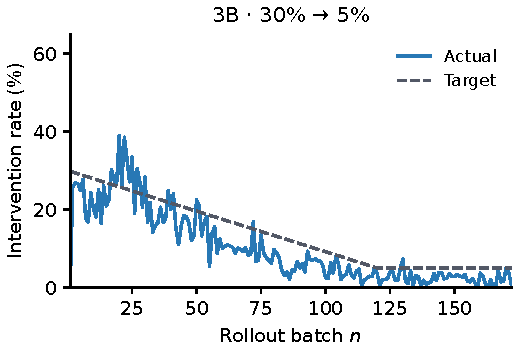
\includegraphics[width=0.48\textwidth]{figures/alfworld_3b_30to5_rate.pdf}\hfill
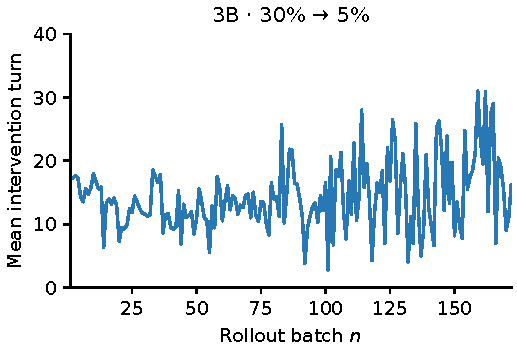
\includegraphics[width=0.48\textwidth]{figures/alfworld_3b_30to5_position.pdf}
\caption{\textbf{Intervention dynamics on ALFWorld with a 3B student and a $30\%\!\to\!5\%$ schedule.}
Left: actual episode-averaged intervention rate (blue) and scheduled target
(dashed gray). Right: mean intervention turn among corrected trajectories.
Interventions become less frequent, while their positions remain variable.}
\label{fig:alfworld-intervention-dynamics}
\end{figure}

